% !TeX root = ../../latex-talk.tex

\part{更进一步}

\begin{frame}
  \frametitle{其他 \LaTeX\ 中文入门资料}
  \begin{bibliolist}{00}
    \onlineitem \textsc{Reckdahl~K.}
    王磊~译.
    \newblock \LaTeX{} 插图指南[EB/OL].
    \newblock 第三版. 2017. \url{https://github.com/WenboSheng/epslatex-cn}.

    \onlineitem 包太雷.
    \newblock \LaTeX\ Notes[EB/OL].
    \newblock 第二版. 2021. \url{https://github.com/huangxg/lnotes}.

    \bookitem 刘海洋.
    \newblock \LaTeX\ 入门[M]. 
    \newblock 北京:电子工业出版社, 2013.
  \end{bibliolist}
\end{frame}

\begin{frame}
  \frametitle{其他 \LaTeX\ 经典资料}
  \begin{bibliolist}{00}
    \onlineitem \textsc{Overleaf}.
    \newblock Learn \LaTeX\ in 30 minutes[EB/OL]. 
    \newblock \url{https://www.overleaf.com/learn/latex/Learn_LaTeX_in_30_minutes}.

    \bookitem \textsc{M.R.C. van Dongen}.
    \newblock \LaTeX{} and Friends[M/OL].
    \newblock New York: Springer, 2012. 
    \url{https://link.springer.com/book/10.1007/978-3-642-23816-1}

    \bookitem \textsc{Mittelbach F.}, \textsc{Goossens M.}, \textsc{Braams J.}, et al.
    \newblock The \LaTeX\ Companion[M].
    \newblock 2nd ed. Boston: Addison-Wesley Professional. 2004.
  \end{bibliolist}
\end{frame}

\begin{frame}
  \frametitle{仍有 \LaTeX\ 的问题?}
  \begin{itemize}
    \item 首先可以查阅宏包的附带文档。在命令行输入
    
    \hfill
    \begin{minipage}{0.3\textwidth}
      \begin{exampleblock}{\faTerminal}
        \ttfamily
        texdoc \textit{<pkg>}
      \end{exampleblock}
    \end{minipage}
    \item 其次可以考虑向 \TeX{} StackExchange \link{https://tex.stackexchange.com/} 寻找解答或提出问题。
    \item 中文相关的问题可以在 \CTeX{} 临时论坛 \link{https://github.com/CTeX-org/forum} 搜寻。
    \item 提问时请附上最小工作案例(MWE)与日志文件。
  \end{itemize}
\end{frame}

\begin{frame}
  \frametitle{敬请期待}
  
  5 月 18 日还会有一讲来讨论 \LaTeX\ 更加注重视觉效果的相关知识。

  \begin{columns}
    \begin{column}{0.5\textwidth}
      \begin{figure}
        \begin{stampbox}[sjtuRedPrimary]
          \includegraphics[height=0.4\textheight]{support/beamer/hello.pdf}
        \end{stampbox}
        \caption{\textsc{SJTUBeamer} \link{https://github.com/sjtug/SJTUBeamer}}
      \end{figure}
    \end{column}
    \begin{column}{0.5\textwidth}
      \begin{figure}
        \begin{stampbox}[sjtuRedPrimary]
          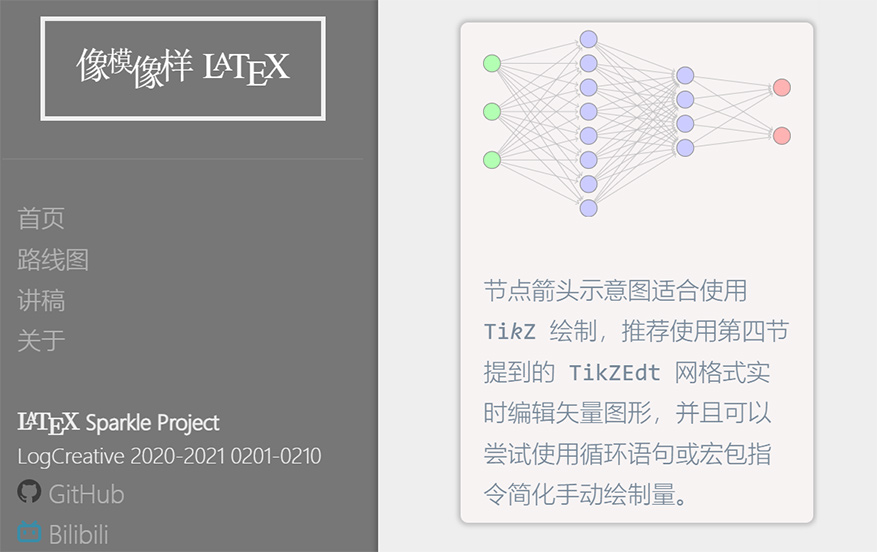
\includegraphics[height=0.4\textheight]{support/images/latexsparkle.jpg}
        \end{stampbox}
        \caption{像模像样 \LaTeX\ \link{https://logcreative.tech/LaTeXSparkle}}
      \end{figure}
    \end{column}
  \end{columns}
\end{frame}